\documentclass[twoside]{book}

% Packages required by doxygen
\usepackage{fixltx2e}
\usepackage{calc}
\usepackage{doxygen}
\usepackage[export]{adjustbox} % also loads graphicx
\usepackage{graphicx}
\usepackage[utf8]{inputenc}
\usepackage{makeidx}
\usepackage{multicol}
\usepackage{multirow}
\PassOptionsToPackage{warn}{textcomp}
\usepackage{textcomp}
\usepackage[nointegrals]{wasysym}
\usepackage[table]{xcolor}

% Font selection
\usepackage[T1]{fontenc}
\usepackage[scaled=.90]{helvet}
\usepackage{courier}
\usepackage{amssymb}
\usepackage{sectsty}
\renewcommand{\familydefault}{\sfdefault}
\allsectionsfont{%
  \fontseries{bc}\selectfont%
  \color{darkgray}%
}
\renewcommand{\DoxyLabelFont}{%
  \fontseries{bc}\selectfont%
  \color{darkgray}%
}
\newcommand{\+}{\discretionary{\mbox{\scriptsize$\hookleftarrow$}}{}{}}

% Page & text layout
\usepackage{geometry}
\geometry{%
  a4paper,%
  top=2.5cm,%
  bottom=2.5cm,%
  left=2.5cm,%
  right=2.5cm%
}
\tolerance=750
\hfuzz=15pt
\hbadness=750
\setlength{\emergencystretch}{15pt}
\setlength{\parindent}{0cm}
\setlength{\parskip}{3ex plus 2ex minus 2ex}
\makeatletter
\renewcommand{\paragraph}{%
  \@startsection{paragraph}{4}{0ex}{-1.0ex}{1.0ex}{%
    \normalfont\normalsize\bfseries\SS@parafont%
  }%
}
\renewcommand{\subparagraph}{%
  \@startsection{subparagraph}{5}{0ex}{-1.0ex}{1.0ex}{%
    \normalfont\normalsize\bfseries\SS@subparafont%
  }%
}
\makeatother

% Headers & footers
\usepackage{fancyhdr}
\pagestyle{fancyplain}
\fancyhead[LE]{\fancyplain{}{\bfseries\thepage}}
\fancyhead[CE]{\fancyplain{}{}}
\fancyhead[RE]{\fancyplain{}{\bfseries\leftmark}}
\fancyhead[LO]{\fancyplain{}{\bfseries\rightmark}}
\fancyhead[CO]{\fancyplain{}{}}
\fancyhead[RO]{\fancyplain{}{\bfseries\thepage}}
\fancyfoot[LE]{\fancyplain{}{}}
\fancyfoot[CE]{\fancyplain{}{}}
\fancyfoot[RE]{\fancyplain{}{\bfseries\scriptsize Generated by Doxygen }}
\fancyfoot[LO]{\fancyplain{}{\bfseries\scriptsize Generated by Doxygen }}
\fancyfoot[CO]{\fancyplain{}{}}
\fancyfoot[RO]{\fancyplain{}{}}
\renewcommand{\footrulewidth}{0.4pt}
\renewcommand{\chaptermark}[1]{%
  \markboth{#1}{}%
}
\renewcommand{\sectionmark}[1]{%
  \markright{\thesection\ #1}%
}

% Indices & bibliography
\usepackage{natbib}
\usepackage[titles]{tocloft}
\setcounter{tocdepth}{3}
\setcounter{secnumdepth}{5}
\makeindex

% Hyperlinks (required, but should be loaded last)
\usepackage{ifpdf}
\ifpdf
  \usepackage[pdftex,pagebackref=true]{hyperref}
\else
  \usepackage[ps2pdf,pagebackref=true]{hyperref}
\fi
\hypersetup{%
  colorlinks=true,%
  linkcolor=blue,%
  citecolor=blue,%
  unicode%
}

% Custom commands
\newcommand{\clearemptydoublepage}{%
  \newpage{\pagestyle{empty}\cleardoublepage}%
}

\usepackage{caption}
\captionsetup{labelsep=space,justification=centering,font={bf},singlelinecheck=off,skip=4pt,position=top}

%===== C O N T E N T S =====

\begin{document}

% Titlepage & ToC
\hypersetup{pageanchor=false,
             bookmarksnumbered=true,
             pdfencoding=unicode
            }
\pagenumbering{alph}
\begin{titlepage}
\vspace*{7cm}
\begin{center}%
{\Large My Project }\\
\vspace*{1cm}
{\large Generated by Doxygen 1.8.14}\\
\end{center}
\end{titlepage}
\clearemptydoublepage
\pagenumbering{roman}
\tableofcontents
\clearemptydoublepage
\pagenumbering{arabic}
\hypersetup{pageanchor=true}

%--- Begin generated contents ---
\chapter{Namespace Index}
\section{Namespace List}
Here is a list of all documented namespaces with brief descriptions\+:\begin{DoxyCompactList}
\item\contentsline{section}{\mbox{\hyperlink{namespacecalculations}{calculations}} }{\pageref{namespacecalculations}}{}
\item\contentsline{section}{\mbox{\hyperlink{namespace_n_o_a_a___monitor}{N\+O\+A\+A\+\_\+\+Monitor}} }{\pageref{namespace_n_o_a_a___monitor}}{}
\item\contentsline{section}{\mbox{\hyperlink{namespacescrape___n_o_a_a__buoy}{scrape\+\_\+\+N\+O\+A\+A\+\_\+buoy}} }{\pageref{namespacescrape___n_o_a_a__buoy}}{}
\end{DoxyCompactList}

\chapter{Hierarchical Index}
\section{Class Hierarchy}
This inheritance list is sorted roughly, but not completely, alphabetically\+:\begin{DoxyCompactList}
\item \contentsline{section}{Buoy}{\pageref{class_buoy}}{}
\item \contentsline{section}{Buoy\+List}{\pageref{class_buoy_list}}{}
\item \contentsline{section}{calculations}{\pageref{classcalculations}}{}
\item \contentsline{section}{calculations.\+calculations}{\pageref{classcalculations_1_1calculations}}{}
\item \contentsline{section}{Graphing}{\pageref{class_graphing}}{}
\item \contentsline{section}{Mapping}{\pageref{class_mapping}}{}
\item Material\+Form\begin{DoxyCompactList}
\item \contentsline{section}{N\+O\+A\+A\+\_\+\+Monitor.\+graph\+Form}{\pageref{class_n_o_a_a___monitor_1_1graph_form}}{}
\item \contentsline{section}{N\+O\+A\+A\+\_\+\+Monitor.\+Main\+Window}{\pageref{class_n_o_a_a___monitor_1_1_main_window}}{}
\end{DoxyCompactList}
\end{DoxyCompactList}

\chapter{Class Index}
\section{Class List}
Here are the classes, structs, unions and interfaces with brief descriptions\+:\begin{DoxyCompactList}
\item\contentsline{section}{\mbox{\hyperlink{class_buoy}{Buoy}} }{\pageref{class_buoy}}{}
\item\contentsline{section}{\mbox{\hyperlink{class_buoy_list}{Buoy\+List}} }{\pageref{class_buoy_list}}{}
\item\contentsline{section}{\mbox{\hyperlink{classcalculations}{calculations}} }{\pageref{classcalculations}}{}
\item\contentsline{section}{\mbox{\hyperlink{classcalculations_1_1calculations}{calculations.\+calculations}} }{\pageref{classcalculations_1_1calculations}}{}
\item\contentsline{section}{\mbox{\hyperlink{class_n_o_a_a___monitor_1_1graph_form}{N\+O\+A\+A\+\_\+\+Monitor.\+graph\+Form}} }{\pageref{class_n_o_a_a___monitor_1_1graph_form}}{}
\item\contentsline{section}{\mbox{\hyperlink{class_graphing}{Graphing}} }{\pageref{class_graphing}}{}
\item\contentsline{section}{\mbox{\hyperlink{class_n_o_a_a___monitor_1_1_main_window}{N\+O\+A\+A\+\_\+\+Monitor.\+Main\+Window}} }{\pageref{class_n_o_a_a___monitor_1_1_main_window}}{}
\item\contentsline{section}{\mbox{\hyperlink{class_mapping}{Mapping}} }{\pageref{class_mapping}}{}
\end{DoxyCompactList}

\chapter{Namespace Documentation}
\hypertarget{namespacecalculations}{}\section{calculations Namespace Reference}
\label{namespacecalculations}\index{calculations@{calculations}}
\subsection*{Classes}
\begin{DoxyCompactItemize}
\item 
class \mbox{\hyperlink{classcalculations_1_1calculations}{calculations}}
\end{DoxyCompactItemize}

\hypertarget{namespace_n_o_a_a___monitor}{}\section{N\+O\+A\+A\+\_\+\+Monitor Namespace Reference}
\label{namespace_n_o_a_a___monitor}\index{N\+O\+A\+A\+\_\+\+Monitor@{N\+O\+A\+A\+\_\+\+Monitor}}
\subsection*{Classes}
\begin{DoxyCompactItemize}
\item 
class \mbox{\hyperlink{class_n_o_a_a___monitor_1_1graph_form}{graph\+Form}}
\item 
class \mbox{\hyperlink{class_n_o_a_a___monitor_1_1_main_window}{Main\+Window}}
\item 
class {\bfseries Program}
\end{DoxyCompactItemize}

\hypertarget{namespacescrape___n_o_a_a__buoy}{}\section{scrape\+\_\+\+N\+O\+A\+A\+\_\+buoy Namespace Reference}
\label{namespacescrape___n_o_a_a__buoy}\index{scrape\+\_\+\+N\+O\+A\+A\+\_\+buoy@{scrape\+\_\+\+N\+O\+A\+A\+\_\+buoy}}
\subsection*{Functions}
\begin{DoxyCompactItemize}
\item 
\mbox{\Hypertarget{namespacescrape___n_o_a_a__buoy_ac1297b9efa5abc85c1661691635c3f41}\label{namespacescrape___n_o_a_a__buoy_ac1297b9efa5abc85c1661691635c3f41}} 
def {\bfseries words} (file\+Obj)
\item 
\mbox{\Hypertarget{namespacescrape___n_o_a_a__buoy_adb1ea63f42f9a21619ae902191575640}\label{namespacescrape___n_o_a_a__buoy_adb1ea63f42f9a21619ae902191575640}} 
def {\bfseries count\+Stations} (file\+Obj)
\end{DoxyCompactItemize}
\subsection*{Variables}
\begin{DoxyCompactItemize}
\item 
\mbox{\Hypertarget{namespacescrape___n_o_a_a__buoy_a13231aceb490b34c59a3ff93ef1f3683}\label{namespacescrape___n_o_a_a__buoy_a13231aceb490b34c59a3ff93ef1f3683}} 
string {\bfseries noaa\+\_\+\+Data\+\_\+url} = \char`\"{}https\+://www.\+ndbc.\+noaa.\+gov/data/latest\+\_\+obs/latest\+\_\+obs.\+txt\char`\"{}
\item 
\mbox{\Hypertarget{namespacescrape___n_o_a_a__buoy_ad05b5be8214b4f2f095a94d7eb589c14}\label{namespacescrape___n_o_a_a__buoy_ad05b5be8214b4f2f095a94d7eb589c14}} 
string {\bfseries single\+\_\+page\+\_\+url} = \char`\"{}https\+://www.\+ndbc.\+noaa.\+gov/station\+\_\+page.\+php?station=M\+D\+R\+M1\char`\"{}
\item 
\mbox{\Hypertarget{namespacescrape___n_o_a_a__buoy_a1c324eb194befae4063a7872336f06f7}\label{namespacescrape___n_o_a_a__buoy_a1c324eb194befae4063a7872336f06f7}} 
{\bfseries u\+Client} = u\+Req(noaa\+\_\+\+Data\+\_\+url)
\item 
\mbox{\Hypertarget{namespacescrape___n_o_a_a__buoy_a03665f0d0faa2bc42bb808ad824ad6e9}\label{namespacescrape___n_o_a_a__buoy_a03665f0d0faa2bc42bb808ad824ad6e9}} 
{\bfseries page\+\_\+raw\+\_\+html} = u\+Client.\+read()
\item 
\mbox{\Hypertarget{namespacescrape___n_o_a_a__buoy_ad178ab153214f14621228a7f719f0f7c}\label{namespacescrape___n_o_a_a__buoy_ad178ab153214f14621228a7f719f0f7c}} 
{\bfseries file} = open(\textquotesingle{}tmp.\+txt\textquotesingle{}, \textquotesingle{}w\textquotesingle{})
\item 
\mbox{\Hypertarget{namespacescrape___n_o_a_a__buoy_a4fcbe090ba99971fef19beafb1a59a31}\label{namespacescrape___n_o_a_a__buoy_a4fcbe090ba99971fef19beafb1a59a31}} 
def {\bfseries lines\+\_\+\+N\+O\+A\+A\+\_\+\+Data} = words(file)
\item 
\mbox{\Hypertarget{namespacescrape___n_o_a_a__buoy_ad05b95e4046291707dcfdf9e3b9451ad}\label{namespacescrape___n_o_a_a__buoy_ad05b95e4046291707dcfdf9e3b9451ad}} 
list {\bfseries attribute\+\_\+list} = \mbox{[}$\,$\mbox{]}
\item 
\mbox{\Hypertarget{namespacescrape___n_o_a_a__buoy_a208ab0f0e1e7dff400c7f4342f71a22b}\label{namespacescrape___n_o_a_a__buoy_a208ab0f0e1e7dff400c7f4342f71a22b}} 
dictionary {\bfseries data} = \{\}
\item 
\mbox{\Hypertarget{namespacescrape___n_o_a_a__buoy_a30858790a57da253c204891135cfed35}\label{namespacescrape___n_o_a_a__buoy_a30858790a57da253c204891135cfed35}} 
def {\bfseries num\+Stations} = count\+Stations(file)
\item 
\mbox{\Hypertarget{namespacescrape___n_o_a_a__buoy_aa1419d157780d68fd320aa068022fe2c}\label{namespacescrape___n_o_a_a__buoy_aa1419d157780d68fd320aa068022fe2c}} 
list {\bfseries word\+\_\+\+N\+O\+A\+A\+\_\+\+Data} = \mbox{[}$\,$\mbox{]}
\item 
\mbox{\Hypertarget{namespacescrape___n_o_a_a__buoy_af236cd277a9ee5dbc44061ad0aee6436}\label{namespacescrape___n_o_a_a__buoy_af236cd277a9ee5dbc44061ad0aee6436}} 
def {\bfseries words\+\_\+\+N\+O\+A\+A\+\_\+\+Data} = words(file)
\item 
\mbox{\Hypertarget{namespacescrape___n_o_a_a__buoy_ac431707bdcfc97de5c4e55620f3edc22}\label{namespacescrape___n_o_a_a__buoy_ac431707bdcfc97de5c4e55620f3edc22}} 
int {\bfseries counter} = 0
\item 
\mbox{\Hypertarget{namespacescrape___n_o_a_a__buoy_acfb5a9032b48342e66c387977e98d0f9}\label{namespacescrape___n_o_a_a__buoy_acfb5a9032b48342e66c387977e98d0f9}} 
{\bfseries json\+File} = open(\char`\"{}latest\+\_\+obs.\+json\char`\"{}, \char`\"{}a\char`\"{})
\item 
\mbox{\Hypertarget{namespacescrape___n_o_a_a__buoy_afd38d2dcc28ce29bd902515fd4f90fb4}\label{namespacescrape___n_o_a_a__buoy_afd38d2dcc28ce29bd902515fd4f90fb4}} 
{\bfseries sort\+\_\+keys}
\item 
\mbox{\Hypertarget{namespacescrape___n_o_a_a__buoy_a4c71c7b66fe80449f261f77161497df4}\label{namespacescrape___n_o_a_a__buoy_a4c71c7b66fe80449f261f77161497df4}} 
{\bfseries False}
\item 
\mbox{\Hypertarget{namespacescrape___n_o_a_a__buoy_a6eca3040dae84a81c50769d2c116e69f}\label{namespacescrape___n_o_a_a__buoy_a6eca3040dae84a81c50769d2c116e69f}} 
{\bfseries indent}
\item 
\mbox{\Hypertarget{namespacescrape___n_o_a_a__buoy_a9bb62d822eeb576e4f5ac831d5cc117b}\label{namespacescrape___n_o_a_a__buoy_a9bb62d822eeb576e4f5ac831d5cc117b}} 
{\bfseries separators}
\end{DoxyCompactItemize}


\subsection{Detailed Description}
\begin{DoxyVerb}DOCSTRING - ...
\end{DoxyVerb}
 
\chapter{Class Documentation}
\hypertarget{class_buoy}{}\section{Buoy Class Reference}
\label{class_buoy}\index{Buoy@{Buoy}}
\subsection*{Public Member Functions}
\begin{DoxyCompactItemize}
\item 
\mbox{\hyperlink{class_buoy_aa6aa319139546405b1590e2ef8a292ae}{Buoy}} ()
\item 
void \mbox{\hyperlink{class_buoy_adebcdc47416100216797efc05dda77a3}{input}} (string ins)
\item 
void \mbox{\hyperlink{class_buoy_a9e5167e5f0967ee99f03ba223236b2d4}{display}} ()
\item 
string \mbox{\hyperlink{class_buoy_a70a9f0c2ed761cb6652de7f5b4d51e8c}{getbname}} ()
\item 
string \mbox{\hyperlink{class_buoy_ace0fbd097bbdd61b32d46e524b93f2eb}{getlatlon}} ()
\item 
string \mbox{\hyperlink{class_buoy_add4f34cc5cf9d4f76e0bef759dddf718}{getdate}} ()
\item 
string \mbox{\hyperlink{class_buoy_a03ceca146a3ccd55a0dfeeda8ae64c9d}{getwindspeed}} ()
\item 
string \mbox{\hyperlink{class_buoy_a9ddb36ab4c43611fc0b863eb0b2df958}{getgustspeed}} ()
\item 
string \mbox{\hyperlink{class_buoy_a94314f54fc596eab0a5cceb72b92725a}{getwaveheight}} ()
\item 
string \mbox{\hyperlink{class_buoy_ae19fe8af463418b675deacedeb7f2747}{getdomwave}} ()
\item 
string \mbox{\hyperlink{class_buoy_a585117182ea30d68098d5b5c0dc7f78c}{getavewave}} ()
\item 
string \mbox{\hyperlink{class_buoy_a665b522593ab478b242dd8a535c9341e}{getwavedir}} ()
\item 
string \mbox{\hyperlink{class_buoy_a487ea32a868903d7239975dd52953c70}{getseapress}} ()
\item 
string \mbox{\hyperlink{class_buoy_ad54dfe539e30d1557b315646e1cb36bd}{getpressten}} ()
\item 
string \mbox{\hyperlink{class_buoy_a72746a5814c47d1d5ec06159cd16fa5e}{getseatemp}} ()
\item 
string \mbox{\hyperlink{class_buoy_a7c7561385cfeb04abb1e40cdf52b9118}{getairtemp}} ()
\item 
string \mbox{\hyperlink{class_buoy_a7b9e88f8edb79946073523fc7acc325c}{getdewtemp}} ()
\item 
string \mbox{\hyperlink{class_buoy_a8688ad14f6a063e07f16e6528f7c759e}{getvis}} ()
\item 
string \mbox{\hyperlink{class_buoy_a4ce29e4567cf7541f078c806c2022c39}{gettide}} ()
\end{DoxyCompactItemize}


\subsection{Constructor \& Destructor Documentation}
\mbox{\Hypertarget{class_buoy_aa6aa319139546405b1590e2ef8a292ae}\label{class_buoy_aa6aa319139546405b1590e2ef8a292ae}} 
\index{Buoy@{Buoy}!Buoy@{Buoy}}
\index{Buoy@{Buoy}!Buoy@{Buoy}}
\subsubsection{\texorpdfstring{Buoy()}{Buoy()}}
{\footnotesize\ttfamily Buoy.\+Buoy (\begin{DoxyParamCaption}{ }\end{DoxyParamCaption})\hspace{0.3cm}{\ttfamily [inline]}}

The constructor 

\subsection{Member Function Documentation}
\mbox{\Hypertarget{class_buoy_a9e5167e5f0967ee99f03ba223236b2d4}\label{class_buoy_a9e5167e5f0967ee99f03ba223236b2d4}} 
\index{Buoy@{Buoy}!display@{display}}
\index{display@{display}!Buoy@{Buoy}}
\subsubsection{\texorpdfstring{display()}{display()}}
{\footnotesize\ttfamily void Buoy.\+display (\begin{DoxyParamCaption}{ }\end{DoxyParamCaption})\hspace{0.3cm}{\ttfamily [inline]}}

Displays all information of the buoy \mbox{\Hypertarget{class_buoy_a7c7561385cfeb04abb1e40cdf52b9118}\label{class_buoy_a7c7561385cfeb04abb1e40cdf52b9118}} 
\index{Buoy@{Buoy}!getairtemp@{getairtemp}}
\index{getairtemp@{getairtemp}!Buoy@{Buoy}}
\subsubsection{\texorpdfstring{getairtemp()}{getairtemp()}}
{\footnotesize\ttfamily string Buoy.\+getairtemp (\begin{DoxyParamCaption}{ }\end{DoxyParamCaption})\hspace{0.3cm}{\ttfamily [inline]}}

Gets the air temperature of the buoy \begin{DoxyReturn}{Returns}
The air temperature 
\end{DoxyReturn}
\mbox{\Hypertarget{class_buoy_a585117182ea30d68098d5b5c0dc7f78c}\label{class_buoy_a585117182ea30d68098d5b5c0dc7f78c}} 
\index{Buoy@{Buoy}!getavewave@{getavewave}}
\index{getavewave@{getavewave}!Buoy@{Buoy}}
\subsubsection{\texorpdfstring{getavewave()}{getavewave()}}
{\footnotesize\ttfamily string Buoy.\+getavewave (\begin{DoxyParamCaption}{ }\end{DoxyParamCaption})\hspace{0.3cm}{\ttfamily [inline]}}

Gets the average wave period of the buoy \begin{DoxyReturn}{Returns}
The average wave period 
\end{DoxyReturn}
\mbox{\Hypertarget{class_buoy_a70a9f0c2ed761cb6652de7f5b4d51e8c}\label{class_buoy_a70a9f0c2ed761cb6652de7f5b4d51e8c}} 
\index{Buoy@{Buoy}!getbname@{getbname}}
\index{getbname@{getbname}!Buoy@{Buoy}}
\subsubsection{\texorpdfstring{getbname()}{getbname()}}
{\footnotesize\ttfamily string Buoy.\+getbname (\begin{DoxyParamCaption}{ }\end{DoxyParamCaption})\hspace{0.3cm}{\ttfamily [inline]}}

Gets the buoy name from the buoy \begin{DoxyReturn}{Returns}
The buoy name 
\end{DoxyReturn}
\mbox{\Hypertarget{class_buoy_add4f34cc5cf9d4f76e0bef759dddf718}\label{class_buoy_add4f34cc5cf9d4f76e0bef759dddf718}} 
\index{Buoy@{Buoy}!getdate@{getdate}}
\index{getdate@{getdate}!Buoy@{Buoy}}
\subsubsection{\texorpdfstring{getdate()}{getdate()}}
{\footnotesize\ttfamily string Buoy.\+getdate (\begin{DoxyParamCaption}{ }\end{DoxyParamCaption})\hspace{0.3cm}{\ttfamily [inline]}}

Gets the date the data was collected from the buoy \begin{DoxyReturn}{Returns}
The date 
\end{DoxyReturn}
\mbox{\Hypertarget{class_buoy_a7b9e88f8edb79946073523fc7acc325c}\label{class_buoy_a7b9e88f8edb79946073523fc7acc325c}} 
\index{Buoy@{Buoy}!getdewtemp@{getdewtemp}}
\index{getdewtemp@{getdewtemp}!Buoy@{Buoy}}
\subsubsection{\texorpdfstring{getdewtemp()}{getdewtemp()}}
{\footnotesize\ttfamily string Buoy.\+getdewtemp (\begin{DoxyParamCaption}{ }\end{DoxyParamCaption})\hspace{0.3cm}{\ttfamily [inline]}}

Gets the dewpoint temperture of the buoy \begin{DoxyReturn}{Returns}
The dewpoint temperature 
\end{DoxyReturn}
\mbox{\Hypertarget{class_buoy_ae19fe8af463418b675deacedeb7f2747}\label{class_buoy_ae19fe8af463418b675deacedeb7f2747}} 
\index{Buoy@{Buoy}!getdomwave@{getdomwave}}
\index{getdomwave@{getdomwave}!Buoy@{Buoy}}
\subsubsection{\texorpdfstring{getdomwave()}{getdomwave()}}
{\footnotesize\ttfamily string Buoy.\+getdomwave (\begin{DoxyParamCaption}{ }\end{DoxyParamCaption})\hspace{0.3cm}{\ttfamily [inline]}}

Gets the dominant wave period of the buoy \begin{DoxyReturn}{Returns}
The dominant wave period 
\end{DoxyReturn}
\mbox{\Hypertarget{class_buoy_a9ddb36ab4c43611fc0b863eb0b2df958}\label{class_buoy_a9ddb36ab4c43611fc0b863eb0b2df958}} 
\index{Buoy@{Buoy}!getgustspeed@{getgustspeed}}
\index{getgustspeed@{getgustspeed}!Buoy@{Buoy}}
\subsubsection{\texorpdfstring{getgustspeed()}{getgustspeed()}}
{\footnotesize\ttfamily string Buoy.\+getgustspeed (\begin{DoxyParamCaption}{ }\end{DoxyParamCaption})\hspace{0.3cm}{\ttfamily [inline]}}

Gets the gust speed of the buoy \begin{DoxyReturn}{Returns}
The gust speed 
\end{DoxyReturn}
\mbox{\Hypertarget{class_buoy_ace0fbd097bbdd61b32d46e524b93f2eb}\label{class_buoy_ace0fbd097bbdd61b32d46e524b93f2eb}} 
\index{Buoy@{Buoy}!getlatlon@{getlatlon}}
\index{getlatlon@{getlatlon}!Buoy@{Buoy}}
\subsubsection{\texorpdfstring{getlatlon()}{getlatlon()}}
{\footnotesize\ttfamily string Buoy.\+getlatlon (\begin{DoxyParamCaption}{ }\end{DoxyParamCaption})\hspace{0.3cm}{\ttfamily [inline]}}

Gets the coordinates of the buoy \begin{DoxyReturn}{Returns}
The latitude and longitude 
\end{DoxyReturn}
\mbox{\Hypertarget{class_buoy_ad54dfe539e30d1557b315646e1cb36bd}\label{class_buoy_ad54dfe539e30d1557b315646e1cb36bd}} 
\index{Buoy@{Buoy}!getpressten@{getpressten}}
\index{getpressten@{getpressten}!Buoy@{Buoy}}
\subsubsection{\texorpdfstring{getpressten()}{getpressten()}}
{\footnotesize\ttfamily string Buoy.\+getpressten (\begin{DoxyParamCaption}{ }\end{DoxyParamCaption})\hspace{0.3cm}{\ttfamily [inline]}}

Gets the pressure tendency of the buoy \begin{DoxyReturn}{Returns}
The pressure tendency 
\end{DoxyReturn}
\mbox{\Hypertarget{class_buoy_a487ea32a868903d7239975dd52953c70}\label{class_buoy_a487ea32a868903d7239975dd52953c70}} 
\index{Buoy@{Buoy}!getseapress@{getseapress}}
\index{getseapress@{getseapress}!Buoy@{Buoy}}
\subsubsection{\texorpdfstring{getseapress()}{getseapress()}}
{\footnotesize\ttfamily string Buoy.\+getseapress (\begin{DoxyParamCaption}{ }\end{DoxyParamCaption})\hspace{0.3cm}{\ttfamily [inline]}}

Gets the sea pressure of the buoy \begin{DoxyReturn}{Returns}
The sea pressure 
\end{DoxyReturn}
\mbox{\Hypertarget{class_buoy_a72746a5814c47d1d5ec06159cd16fa5e}\label{class_buoy_a72746a5814c47d1d5ec06159cd16fa5e}} 
\index{Buoy@{Buoy}!getseatemp@{getseatemp}}
\index{getseatemp@{getseatemp}!Buoy@{Buoy}}
\subsubsection{\texorpdfstring{getseatemp()}{getseatemp()}}
{\footnotesize\ttfamily string Buoy.\+getseatemp (\begin{DoxyParamCaption}{ }\end{DoxyParamCaption})\hspace{0.3cm}{\ttfamily [inline]}}

Gets the sea temperature of the buoy \begin{DoxyReturn}{Returns}
The sea temperature 
\end{DoxyReturn}
\mbox{\Hypertarget{class_buoy_a4ce29e4567cf7541f078c806c2022c39}\label{class_buoy_a4ce29e4567cf7541f078c806c2022c39}} 
\index{Buoy@{Buoy}!gettide@{gettide}}
\index{gettide@{gettide}!Buoy@{Buoy}}
\subsubsection{\texorpdfstring{gettide()}{gettide()}}
{\footnotesize\ttfamily string Buoy.\+gettide (\begin{DoxyParamCaption}{ }\end{DoxyParamCaption})\hspace{0.3cm}{\ttfamily [inline]}}

Gets the water level of the buoy \begin{DoxyReturn}{Returns}
The water level 
\end{DoxyReturn}
\mbox{\Hypertarget{class_buoy_a8688ad14f6a063e07f16e6528f7c759e}\label{class_buoy_a8688ad14f6a063e07f16e6528f7c759e}} 
\index{Buoy@{Buoy}!getvis@{getvis}}
\index{getvis@{getvis}!Buoy@{Buoy}}
\subsubsection{\texorpdfstring{getvis()}{getvis()}}
{\footnotesize\ttfamily string Buoy.\+getvis (\begin{DoxyParamCaption}{ }\end{DoxyParamCaption})\hspace{0.3cm}{\ttfamily [inline]}}

Gets the visibility of the buoy \begin{DoxyReturn}{Returns}
The visibility 
\end{DoxyReturn}
\mbox{\Hypertarget{class_buoy_a665b522593ab478b242dd8a535c9341e}\label{class_buoy_a665b522593ab478b242dd8a535c9341e}} 
\index{Buoy@{Buoy}!getwavedir@{getwavedir}}
\index{getwavedir@{getwavedir}!Buoy@{Buoy}}
\subsubsection{\texorpdfstring{getwavedir()}{getwavedir()}}
{\footnotesize\ttfamily string Buoy.\+getwavedir (\begin{DoxyParamCaption}{ }\end{DoxyParamCaption})\hspace{0.3cm}{\ttfamily [inline]}}

Gets the wave direction of the buoy \begin{DoxyReturn}{Returns}
The wave direction 
\end{DoxyReturn}
\mbox{\Hypertarget{class_buoy_a94314f54fc596eab0a5cceb72b92725a}\label{class_buoy_a94314f54fc596eab0a5cceb72b92725a}} 
\index{Buoy@{Buoy}!getwaveheight@{getwaveheight}}
\index{getwaveheight@{getwaveheight}!Buoy@{Buoy}}
\subsubsection{\texorpdfstring{getwaveheight()}{getwaveheight()}}
{\footnotesize\ttfamily string Buoy.\+getwaveheight (\begin{DoxyParamCaption}{ }\end{DoxyParamCaption})\hspace{0.3cm}{\ttfamily [inline]}}

Gets the wave height of the buoy \begin{DoxyReturn}{Returns}
The wave height 
\end{DoxyReturn}
\mbox{\Hypertarget{class_buoy_a03ceca146a3ccd55a0dfeeda8ae64c9d}\label{class_buoy_a03ceca146a3ccd55a0dfeeda8ae64c9d}} 
\index{Buoy@{Buoy}!getwindspeed@{getwindspeed}}
\index{getwindspeed@{getwindspeed}!Buoy@{Buoy}}
\subsubsection{\texorpdfstring{getwindspeed()}{getwindspeed()}}
{\footnotesize\ttfamily string Buoy.\+getwindspeed (\begin{DoxyParamCaption}{ }\end{DoxyParamCaption})\hspace{0.3cm}{\ttfamily [inline]}}

Gets the wind speed of the buoy \begin{DoxyReturn}{Returns}
The wind speed 
\end{DoxyReturn}
\mbox{\Hypertarget{class_buoy_adebcdc47416100216797efc05dda77a3}\label{class_buoy_adebcdc47416100216797efc05dda77a3}} 
\index{Buoy@{Buoy}!input@{input}}
\index{input@{input}!Buoy@{Buoy}}
\subsubsection{\texorpdfstring{input()}{input()}}
{\footnotesize\ttfamily void Buoy.\+input (\begin{DoxyParamCaption}\item[{string}]{ins }\end{DoxyParamCaption})\hspace{0.3cm}{\ttfamily [inline]}}

Inputs a line of data into the buoy 
\begin{DoxyParams}{Parameters}
{\em A} & full line from an input file with all the data for a single buoy \\
\hline
\end{DoxyParams}


The documentation for this class was generated from the following file\+:\begin{DoxyCompactItemize}
\item 
Buoy.\+cs\end{DoxyCompactItemize}

\hypertarget{class_buoy_list}{}\section{Buoy\+List Class Reference}
\label{class_buoy_list}\index{Buoy\+List@{Buoy\+List}}
\subsection*{Public Member Functions}
\begin{DoxyCompactItemize}
\item 
\mbox{\hyperlink{class_buoy_list_a39b03994875a552bdb1087caa2d6b431}{Buoy\+List}} ()
\item 
void \mbox{\hyperlink{class_buoy_list_a5e6195c4558add60568a3fcc12888662}{load}} (string file)
\item 
void \mbox{\hyperlink{class_buoy_list_ac25d70b5e55ad4ce113a1fc26c14b2f0}{bdisplay}} (int index)
\item 
void \mbox{\hyperlink{class_buoy_list_a8e7b3aae97170c455e436a6924947e9b}{search}} (string target)
\item 
\mbox{\hyperlink{class_buoy_list_afedfe1b7d724da215430042550790747}{Buoy\+List}} (\mbox{\hyperlink{class_buoy_list}{Buoy\+List}} a)
\end{DoxyCompactItemize}


\subsection{Constructor \& Destructor Documentation}
\mbox{\Hypertarget{class_buoy_list_a39b03994875a552bdb1087caa2d6b431}\label{class_buoy_list_a39b03994875a552bdb1087caa2d6b431}} 
\index{Buoy\+List@{Buoy\+List}!Buoy\+List@{Buoy\+List}}
\index{Buoy\+List@{Buoy\+List}!Buoy\+List@{Buoy\+List}}
\subsubsection{\texorpdfstring{Buoy\+List()}{BuoyList()}\hspace{0.1cm}{\footnotesize\ttfamily [1/2]}}
{\footnotesize\ttfamily Buoy\+List.\+Buoy\+List (\begin{DoxyParamCaption}{ }\end{DoxyParamCaption})\hspace{0.3cm}{\ttfamily [inline]}}

The constructor of the class \mbox{\Hypertarget{class_buoy_list_afedfe1b7d724da215430042550790747}\label{class_buoy_list_afedfe1b7d724da215430042550790747}} 
\index{Buoy\+List@{Buoy\+List}!Buoy\+List@{Buoy\+List}}
\index{Buoy\+List@{Buoy\+List}!Buoy\+List@{Buoy\+List}}
\subsubsection{\texorpdfstring{Buoy\+List()}{BuoyList()}\hspace{0.1cm}{\footnotesize\ttfamily [2/2]}}
{\footnotesize\ttfamily Buoy\+List.\+Buoy\+List (\begin{DoxyParamCaption}\item[{\mbox{\hyperlink{class_buoy_list}{Buoy\+List}}}]{a }\end{DoxyParamCaption})\hspace{0.3cm}{\ttfamily [inline]}}

Copy constructor 
\begin{DoxyParams}{Parameters}
{\em buoy} & list to be copied from \\
\hline
\end{DoxyParams}


\subsection{Member Function Documentation}
\mbox{\Hypertarget{class_buoy_list_ac25d70b5e55ad4ce113a1fc26c14b2f0}\label{class_buoy_list_ac25d70b5e55ad4ce113a1fc26c14b2f0}} 
\index{Buoy\+List@{Buoy\+List}!bdisplay@{bdisplay}}
\index{bdisplay@{bdisplay}!Buoy\+List@{Buoy\+List}}
\subsubsection{\texorpdfstring{bdisplay()}{bdisplay()}}
{\footnotesize\ttfamily void Buoy\+List.\+bdisplay (\begin{DoxyParamCaption}\item[{int}]{index }\end{DoxyParamCaption})\hspace{0.3cm}{\ttfamily [inline]}}

Displays the information about a buoy 
\begin{DoxyParams}{Parameters}
{\em The} & index of the buoy list to be displayed \\
\hline
\end{DoxyParams}
\mbox{\Hypertarget{class_buoy_list_a5e6195c4558add60568a3fcc12888662}\label{class_buoy_list_a5e6195c4558add60568a3fcc12888662}} 
\index{Buoy\+List@{Buoy\+List}!load@{load}}
\index{load@{load}!Buoy\+List@{Buoy\+List}}
\subsubsection{\texorpdfstring{load()}{load()}}
{\footnotesize\ttfamily void Buoy\+List.\+load (\begin{DoxyParamCaption}\item[{string}]{file }\end{DoxyParamCaption})\hspace{0.3cm}{\ttfamily [inline]}}

Loads from the text file into a list of buoys 
\begin{DoxyParams}{Parameters}
{\em The} & filename of the input file, preferably a text file \\
\hline
\end{DoxyParams}
\mbox{\Hypertarget{class_buoy_list_a8e7b3aae97170c455e436a6924947e9b}\label{class_buoy_list_a8e7b3aae97170c455e436a6924947e9b}} 
\index{Buoy\+List@{Buoy\+List}!search@{search}}
\index{search@{search}!Buoy\+List@{Buoy\+List}}
\subsubsection{\texorpdfstring{search()}{search()}}
{\footnotesize\ttfamily void Buoy\+List.\+search (\begin{DoxyParamCaption}\item[{string}]{target }\end{DoxyParamCaption})\hspace{0.3cm}{\ttfamily [inline]}}

Searches through the list for a specific buoy 
\begin{DoxyParams}{Parameters}
{\em The} & ID (banme) of the buoy to be searched \\
\hline
\end{DoxyParams}


The documentation for this class was generated from the following file\+:\begin{DoxyCompactItemize}
\item 
buoylist.\+cs\end{DoxyCompactItemize}

\hypertarget{classcalculations}{}\section{calculations Class Reference}
\label{classcalculations}\index{calculations@{calculations}}
\subsection*{Public Member Functions}
\begin{DoxyCompactItemize}
\item 
\mbox{\Hypertarget{classcalculations_af034c194e1aac225dd4210b93b8437fe}\label{classcalculations_af034c194e1aac225dd4210b93b8437fe}} 
double {\bfseries celcius\+\_\+to\+\_\+farenheit} (double faren\+\_\+temp)
\item 
\mbox{\Hypertarget{classcalculations_ab10b39ff1b94a54db267b039703f7dc9}\label{classcalculations_ab10b39ff1b94a54db267b039703f7dc9}} 
double {\bfseries farenheit\+\_\+to\+\_\+celcius} (double cel\+\_\+temp)
\item 
\mbox{\Hypertarget{classcalculations_a84b7a97de918305835dc6daea5eea276}\label{classcalculations_a84b7a97de918305835dc6daea5eea276}} 
double {\bfseries vapor\+\_\+pressure} (double air\+\_\+temp)
\item 
\mbox{\Hypertarget{classcalculations_a0b1e2a8224889570ccf12f839dcc0f4e}\label{classcalculations_a0b1e2a8224889570ccf12f839dcc0f4e}} 
double {\bfseries saturated\+\_\+vapor\+\_\+pressure} (double dew\+\_\+point\+\_\+temp)
\item 
\mbox{\Hypertarget{classcalculations_a1ac5cde006b41ccf3eb4169244e7f071}\label{classcalculations_a1ac5cde006b41ccf3eb4169244e7f071}} 
double {\bfseries water\+\_\+temp} (double air\+\_\+temp, double dew\+\_\+point\+\_\+temp, double air\+\_\+pressure)
\item 
\mbox{\Hypertarget{classcalculations_abf4c45e715e32b863bc67340aa89c744}\label{classcalculations_abf4c45e715e32b863bc67340aa89c744}} 
double {\bfseries dew\+\_\+point} (double relative\+\_\+humid, double vap\+\_\+pressure)
\item 
\mbox{\Hypertarget{classcalculations_a38d24a8af0dd39702bab2888acf2e020}\label{classcalculations_a38d24a8af0dd39702bab2888acf2e020}} 
double {\bfseries relative\+\_\+humidity} (double sat\+\_\+vap\+\_\+pressure, double vap\+\_\+pressure)
\end{DoxyCompactItemize}
\subsection*{Public Attributes}
\begin{DoxyCompactItemize}
\item 
\mbox{\Hypertarget{classcalculations_ab91a4811df6f354527e51b177f0f2695}\label{classcalculations_ab91a4811df6f354527e51b177f0f2695}} 
double {\bfseries cel\+\_\+temp}
\item 
\mbox{\Hypertarget{classcalculations_aff43769ef6563aa40705c3cabc757726}\label{classcalculations_aff43769ef6563aa40705c3cabc757726}} 
double {\bfseries faren\+\_\+temp}
\item 
\mbox{\Hypertarget{classcalculations_ab8c2bf801e553f6b6becfa7ead6fc637}\label{classcalculations_ab8c2bf801e553f6b6becfa7ead6fc637}} 
double {\bfseries air\+\_\+temp}
\item 
\mbox{\Hypertarget{classcalculations_ae71819d3ad2561442299690d75998e42}\label{classcalculations_ae71819d3ad2561442299690d75998e42}} 
double {\bfseries dew\+\_\+point\+\_\+temp}
\item 
\mbox{\Hypertarget{classcalculations_a144adda843a20573360cfbdbef58423a}\label{classcalculations_a144adda843a20573360cfbdbef58423a}} 
double {\bfseries relative\+\_\+humid}
\item 
\mbox{\Hypertarget{classcalculations_accf3419d1ccf8dede14c732c991f775e}\label{classcalculations_accf3419d1ccf8dede14c732c991f775e}} 
double {\bfseries vap\+\_\+pressure}
\item 
\mbox{\Hypertarget{classcalculations_a60df1762a9eea5a8e5d81aea36a8e93d}\label{classcalculations_a60df1762a9eea5a8e5d81aea36a8e93d}} 
double {\bfseries sat\+\_\+vap\+\_\+pressure}
\end{DoxyCompactItemize}


The documentation for this class was generated from the following files\+:\begin{DoxyCompactItemize}
\item 
calculations.\+h\item 
calculations.\+cpp\end{DoxyCompactItemize}

\hypertarget{classcalculations_1_1calculations}{}\section{calculations.\+calculations Class Reference}
\label{classcalculations_1_1calculations}\index{calculations.\+calculations@{calculations.\+calculations}}
\subsection*{Public Member Functions}
\begin{DoxyCompactItemize}
\item 
double \mbox{\hyperlink{classcalculations_1_1calculations_ab85048dd6fa5d535ea173d996b3968c1}{farenheit\+\_\+to\+\_\+celcius}} (double faren\+\_\+temp)
\item 
double \mbox{\hyperlink{classcalculations_1_1calculations_a263a1903afa9a2de7221d69feb45d379}{celcius\+\_\+to\+\_\+farenheit}} (double cel\+\_\+temp)
\item 
double \mbox{\hyperlink{classcalculations_1_1calculations_af2e526ba0ac77a303d9b458c2642e5f4}{vapor\+\_\+pressure}} (double air\+\_\+temp)
\item 
double \mbox{\hyperlink{classcalculations_1_1calculations_a2b7da37ed1c95d9894ac9dff614db9e7}{saturated\+\_\+vapor\+\_\+pressure}} (double dew\+\_\+point\+\_\+temp)
\item 
double \mbox{\hyperlink{classcalculations_1_1calculations_ae71bcea53dda2efe2673f2a4897ab684}{water\+\_\+temp}} (double air\+\_\+temp, double dew\+\_\+point\+\_\+temp, double air\+\_\+pressure)
\item 
double \mbox{\hyperlink{classcalculations_1_1calculations_a37b4b4129f95710ac3ed3598d749971c}{dew\+\_\+point}} (double relative\+\_\+humid, double vap\+\_\+pressure)
\item 
double \mbox{\hyperlink{classcalculations_1_1calculations_a9577ccf9df8aeea64ea3fa629bc0ea71}{relative\+\_\+humidity}} (double sat\+\_\+vap\+\_\+pressure, double vap\+\_\+pressure)
\end{DoxyCompactItemize}


\subsection{Detailed Description}
Class for all of the calculations being used to find missing values from the buoy data 

\subsection{Member Function Documentation}
\mbox{\Hypertarget{classcalculations_1_1calculations_a263a1903afa9a2de7221d69feb45d379}\label{classcalculations_1_1calculations_a263a1903afa9a2de7221d69feb45d379}} 
\index{calculations\+::calculations@{calculations\+::calculations}!celcius\+\_\+to\+\_\+farenheit@{celcius\+\_\+to\+\_\+farenheit}}
\index{celcius\+\_\+to\+\_\+farenheit@{celcius\+\_\+to\+\_\+farenheit}!calculations\+::calculations@{calculations\+::calculations}}
\subsubsection{\texorpdfstring{celcius\+\_\+to\+\_\+farenheit()}{celcius\_to\_farenheit()}}
{\footnotesize\ttfamily double calculations.\+calculations.\+celcius\+\_\+to\+\_\+farenheit (\begin{DoxyParamCaption}\item[{double}]{cel\+\_\+temp }\end{DoxyParamCaption})\hspace{0.3cm}{\ttfamily [inline]}}

Function to change from celcius to farenheit 
\begin{DoxyParams}{Parameters}
{\em cel\+\_\+temp} & is the celcius temperature being converted to farenheit \\
\hline
\end{DoxyParams}
\begin{DoxyReturn}{Returns}
returns a double which is the farenheit temperature converted from the given celcius temperature 
\end{DoxyReturn}
\mbox{\Hypertarget{classcalculations_1_1calculations_a37b4b4129f95710ac3ed3598d749971c}\label{classcalculations_1_1calculations_a37b4b4129f95710ac3ed3598d749971c}} 
\index{calculations\+::calculations@{calculations\+::calculations}!dew\+\_\+point@{dew\+\_\+point}}
\index{dew\+\_\+point@{dew\+\_\+point}!calculations\+::calculations@{calculations\+::calculations}}
\subsubsection{\texorpdfstring{dew\+\_\+point()}{dew\_point()}}
{\footnotesize\ttfamily double calculations.\+calculations.\+dew\+\_\+point (\begin{DoxyParamCaption}\item[{double}]{relative\+\_\+humid,  }\item[{double}]{vap\+\_\+pressure }\end{DoxyParamCaption})\hspace{0.3cm}{\ttfamily [inline]}}

Function to calculate the dew point 
\begin{DoxyParams}{Parameters}
{\em relative\+\_\+humid} & is the relative humidity used in calculating the dew point \\
\hline
{\em vap\+\_\+pressure} & is the vapor pressure used in calculating dew point \\
\hline
\end{DoxyParams}
\begin{DoxyReturn}{Returns}
returns the dew point calculated from the given relative\+\_\+humid, and vap\+\_\+pressure 
\end{DoxyReturn}
\mbox{\Hypertarget{classcalculations_1_1calculations_ab85048dd6fa5d535ea173d996b3968c1}\label{classcalculations_1_1calculations_ab85048dd6fa5d535ea173d996b3968c1}} 
\index{calculations\+::calculations@{calculations\+::calculations}!farenheit\+\_\+to\+\_\+celcius@{farenheit\+\_\+to\+\_\+celcius}}
\index{farenheit\+\_\+to\+\_\+celcius@{farenheit\+\_\+to\+\_\+celcius}!calculations\+::calculations@{calculations\+::calculations}}
\subsubsection{\texorpdfstring{farenheit\+\_\+to\+\_\+celcius()}{farenheit\_to\_celcius()}}
{\footnotesize\ttfamily double calculations.\+calculations.\+farenheit\+\_\+to\+\_\+celcius (\begin{DoxyParamCaption}\item[{double}]{faren\+\_\+temp }\end{DoxyParamCaption})\hspace{0.3cm}{\ttfamily [inline]}}

Function to change from farenheit to celcius 
\begin{DoxyParams}{Parameters}
{\em faren\+\_\+temp} & is the farenheit temperature being converted to celcius \\
\hline
\end{DoxyParams}
\begin{DoxyReturn}{Returns}
returns a double which is the celcius temperature converted from the given farenheit temperature 
\end{DoxyReturn}
\mbox{\Hypertarget{classcalculations_1_1calculations_a9577ccf9df8aeea64ea3fa629bc0ea71}\label{classcalculations_1_1calculations_a9577ccf9df8aeea64ea3fa629bc0ea71}} 
\index{calculations\+::calculations@{calculations\+::calculations}!relative\+\_\+humidity@{relative\+\_\+humidity}}
\index{relative\+\_\+humidity@{relative\+\_\+humidity}!calculations\+::calculations@{calculations\+::calculations}}
\subsubsection{\texorpdfstring{relative\+\_\+humidity()}{relative\_humidity()}}
{\footnotesize\ttfamily double calculations.\+calculations.\+relative\+\_\+humidity (\begin{DoxyParamCaption}\item[{double}]{sat\+\_\+vap\+\_\+pressure,  }\item[{double}]{vap\+\_\+pressure }\end{DoxyParamCaption})\hspace{0.3cm}{\ttfamily [inline]}}

Function to calculate the relative humidity 
\begin{DoxyParams}{Parameters}
{\em sat\+\_\+vap\+\_\+pressure} & is the saturated vapor pressure used in calculating the relative humidity \\
\hline
{\em vap\+\_\+pressure} & is the vapor pressure used in calculatin the relative humidity \\
\hline
\end{DoxyParams}
\begin{DoxyReturn}{Returns}
returns the calculated relative humidity calculated from the given saturated vapor pressure, and vapor pressure 
\end{DoxyReturn}
\mbox{\Hypertarget{classcalculations_1_1calculations_a2b7da37ed1c95d9894ac9dff614db9e7}\label{classcalculations_1_1calculations_a2b7da37ed1c95d9894ac9dff614db9e7}} 
\index{calculations\+::calculations@{calculations\+::calculations}!saturated\+\_\+vapor\+\_\+pressure@{saturated\+\_\+vapor\+\_\+pressure}}
\index{saturated\+\_\+vapor\+\_\+pressure@{saturated\+\_\+vapor\+\_\+pressure}!calculations\+::calculations@{calculations\+::calculations}}
\subsubsection{\texorpdfstring{saturated\+\_\+vapor\+\_\+pressure()}{saturated\_vapor\_pressure()}}
{\footnotesize\ttfamily double calculations.\+calculations.\+saturated\+\_\+vapor\+\_\+pressure (\begin{DoxyParamCaption}\item[{double}]{dew\+\_\+point\+\_\+temp }\end{DoxyParamCaption})\hspace{0.3cm}{\ttfamily [inline]}}

Function to calculate the saturated vapor pressureusing the dew point temperature 
\begin{DoxyParams}{Parameters}
{\em dew\+\_\+point\+\_\+temp} & is the dew point temperature used to calculate the saturated vapor pressure \\
\hline
\end{DoxyParams}
\begin{DoxyReturn}{Returns}
returns the calculated saturated vapor pressure from the given dew point temperature 
\end{DoxyReturn}
\mbox{\Hypertarget{classcalculations_1_1calculations_af2e526ba0ac77a303d9b458c2642e5f4}\label{classcalculations_1_1calculations_af2e526ba0ac77a303d9b458c2642e5f4}} 
\index{calculations\+::calculations@{calculations\+::calculations}!vapor\+\_\+pressure@{vapor\+\_\+pressure}}
\index{vapor\+\_\+pressure@{vapor\+\_\+pressure}!calculations\+::calculations@{calculations\+::calculations}}
\subsubsection{\texorpdfstring{vapor\+\_\+pressure()}{vapor\_pressure()}}
{\footnotesize\ttfamily double calculations.\+calculations.\+vapor\+\_\+pressure (\begin{DoxyParamCaption}\item[{double}]{air\+\_\+temp }\end{DoxyParamCaption})\hspace{0.3cm}{\ttfamily [inline]}}

Function to calculate the vapor pressure 
\begin{DoxyParams}{Parameters}
{\em air\+\_\+temp} & is the air temperature used to calculate the vapor pressure \\
\hline
\end{DoxyParams}
\begin{DoxyReturn}{Returns}
returns the calculated vapor pressure from the given air temperature 
\end{DoxyReturn}
\mbox{\Hypertarget{classcalculations_1_1calculations_ae71bcea53dda2efe2673f2a4897ab684}\label{classcalculations_1_1calculations_ae71bcea53dda2efe2673f2a4897ab684}} 
\index{calculations\+::calculations@{calculations\+::calculations}!water\+\_\+temp@{water\+\_\+temp}}
\index{water\+\_\+temp@{water\+\_\+temp}!calculations\+::calculations@{calculations\+::calculations}}
\subsubsection{\texorpdfstring{water\+\_\+temp()}{water\_temp()}}
{\footnotesize\ttfamily double calculations.\+calculations.\+water\+\_\+temp (\begin{DoxyParamCaption}\item[{double}]{air\+\_\+temp,  }\item[{double}]{dew\+\_\+point\+\_\+temp,  }\item[{double}]{air\+\_\+pressure }\end{DoxyParamCaption})\hspace{0.3cm}{\ttfamily [inline]}}

Function to caluculate the water temperature 
\begin{DoxyParams}{Parameters}
{\em air\+\_\+temp} & is the air temperature used to caluclate water temperature \\
\hline
{\em dew\+\_\+point\+\_\+temp} & is the dew point temperature used to calculate water temperature \\
\hline
{\em air\+\_\+pressure} & is the air pressure used to calculate the water temperature \\
\hline
\end{DoxyParams}
\begin{DoxyReturn}{Returns}
returns the water temperature calculated from the given air temperature, dew point temperature, and air pressure 
\end{DoxyReturn}


The documentation for this class was generated from the following file\+:\begin{DoxyCompactItemize}
\item 
Calculations.\+cs\end{DoxyCompactItemize}

\hypertarget{class_n_o_a_a___monitor_1_1graph_form}{}\section{N\+O\+A\+A\+\_\+\+Monitor.\+graph\+Form Class Reference}
\label{class_n_o_a_a___monitor_1_1graph_form}\index{N\+O\+A\+A\+\_\+\+Monitor.\+graph\+Form@{N\+O\+A\+A\+\_\+\+Monitor.\+graph\+Form}}
Inheritance diagram for N\+O\+A\+A\+\_\+\+Monitor.\+graph\+Form\+:\begin{figure}[H]
\begin{center}
\leavevmode
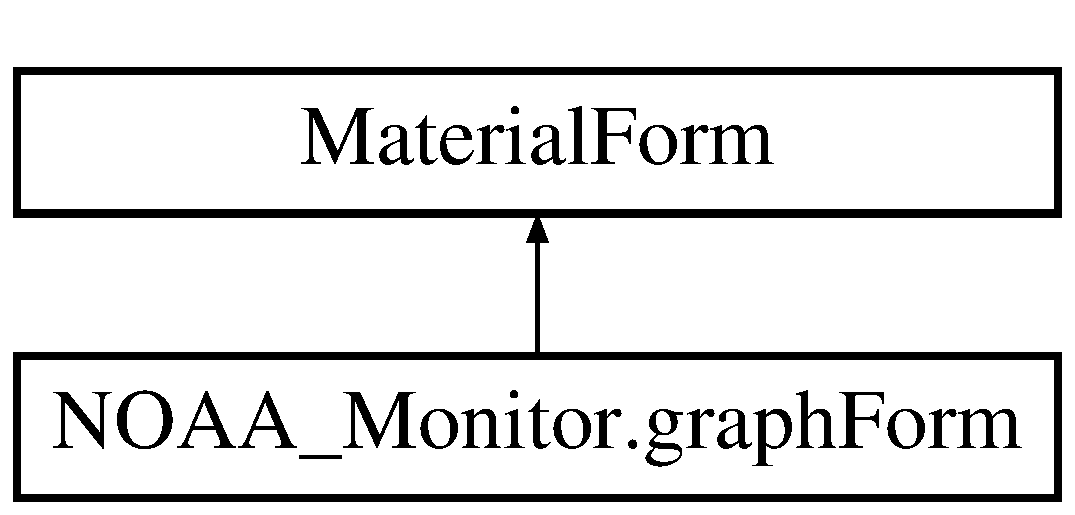
\includegraphics[height=2.000000cm]{class_n_o_a_a___monitor_1_1graph_form}
\end{center}
\end{figure}
\subsection*{Public Member Functions}
\begin{DoxyCompactItemize}
\item 
\mbox{\hyperlink{class_n_o_a_a___monitor_1_1graph_form_a68c6d68e2948df9bc77d6f3d097ee069}{graph\+Form}} (\mbox{\hyperlink{class_buoy_list}{Buoy\+List}} tmp)
\item 
void \mbox{\hyperlink{class_n_o_a_a___monitor_1_1graph_form_a3bad905cbd2cc4f92c5198943d3e3339}{wind\+Speed\+Text}} ()
\item 
void \mbox{\hyperlink{class_n_o_a_a___monitor_1_1graph_form_a88390ff163a7aef5b5f5a653f2b3452e}{wind\+Direction\+Text}} ()
\item 
void \mbox{\hyperlink{class_n_o_a_a___monitor_1_1graph_form_aff28dc3c6bea6ba1fc33f0620c83a277}{dominant\+Wave\+Period\+Text}} ()
\item 
void \mbox{\hyperlink{class_n_o_a_a___monitor_1_1graph_form_ad03af9421d83d6b59ea3a95852a818dd}{average\+Wave\+Period\+Text}} ()
\item 
void \mbox{\hyperlink{class_n_o_a_a___monitor_1_1graph_form_a4b7a6e4f7b99e2cdd178c2755d593a36}{sea\+Pressure\+Text}} ()
\item 
void \mbox{\hyperlink{class_n_o_a_a___monitor_1_1graph_form_a9a7c2bc645a76256d6326777e258f5da}{air\+Temperature\+Text}} ()
\item 
void \mbox{\hyperlink{class_n_o_a_a___monitor_1_1graph_form_a84b5aeb8cb6c0f75289859f7a8d35a3b}{sea\+Temperature\+Text}} ()
\item 
void \mbox{\hyperlink{class_n_o_a_a___monitor_1_1graph_form_ab43bde183f09b6f4a854c361890265f3}{dew\+Temperature\+Text}} ()
\item 
void \mbox{\hyperlink{class_n_o_a_a___monitor_1_1graph_form_a3501fbf78761a0d1ff1a9a22326355ba}{visibility\+Text}} ()
\item 
void \mbox{\hyperlink{class_n_o_a_a___monitor_1_1graph_form_ae941bbbf25f512fddd3dad5cb74437d2}{tide\+Height\+Text}} ()
\end{DoxyCompactItemize}
\subsection*{Protected Member Functions}
\begin{DoxyCompactItemize}
\item 
override void \mbox{\hyperlink{class_n_o_a_a___monitor_1_1graph_form_af498ca1601a85b6ed47927f609d4cb80}{Dispose}} (bool disposing)
\begin{DoxyCompactList}\small\item\em Clean up any resources being used. \end{DoxyCompactList}\end{DoxyCompactItemize}


\subsection{Detailed Description}
This is the implementation of the graphing form class which inherits the Material\+Form class 

\subsection{Constructor \& Destructor Documentation}
\mbox{\Hypertarget{class_n_o_a_a___monitor_1_1graph_form_a68c6d68e2948df9bc77d6f3d097ee069}\label{class_n_o_a_a___monitor_1_1graph_form_a68c6d68e2948df9bc77d6f3d097ee069}} 
\index{N\+O\+A\+A\+\_\+\+Monitor\+::graph\+Form@{N\+O\+A\+A\+\_\+\+Monitor\+::graph\+Form}!graph\+Form@{graph\+Form}}
\index{graph\+Form@{graph\+Form}!N\+O\+A\+A\+\_\+\+Monitor\+::graph\+Form@{N\+O\+A\+A\+\_\+\+Monitor\+::graph\+Form}}
\subsubsection{\texorpdfstring{graph\+Form()}{graphForm()}}
{\footnotesize\ttfamily N\+O\+A\+A\+\_\+\+Monitor.\+graph\+Form.\+graph\+Form (\begin{DoxyParamCaption}\item[{\mbox{\hyperlink{class_buoy_list}{Buoy\+List}}}]{tmp }\end{DoxyParamCaption})\hspace{0.3cm}{\ttfamily [inline]}}

This is the constructor for the \mbox{\hyperlink{class_n_o_a_a___monitor_1_1graph_form}{graph\+Form}} class 
\begin{DoxyParams}{Parameters}
{\em tmp} & is a temporary variable to transfer a \mbox{\hyperlink{class_buoy_list}{Buoy\+List}} variable into the space of this class to be used for graphing \\
\hline
\end{DoxyParams}


\subsection{Member Function Documentation}
\mbox{\Hypertarget{class_n_o_a_a___monitor_1_1graph_form_a9a7c2bc645a76256d6326777e258f5da}\label{class_n_o_a_a___monitor_1_1graph_form_a9a7c2bc645a76256d6326777e258f5da}} 
\index{N\+O\+A\+A\+\_\+\+Monitor\+::graph\+Form@{N\+O\+A\+A\+\_\+\+Monitor\+::graph\+Form}!air\+Temperature\+Text@{air\+Temperature\+Text}}
\index{air\+Temperature\+Text@{air\+Temperature\+Text}!N\+O\+A\+A\+\_\+\+Monitor\+::graph\+Form@{N\+O\+A\+A\+\_\+\+Monitor\+::graph\+Form}}
\subsubsection{\texorpdfstring{air\+Temperature\+Text()}{airTemperatureText()}}
{\footnotesize\ttfamily void N\+O\+A\+A\+\_\+\+Monitor.\+graph\+Form.\+air\+Temperature\+Text (\begin{DoxyParamCaption}{ }\end{DoxyParamCaption})\hspace{0.3cm}{\ttfamily [inline]}}

This prints out the text for the air temperature graph \mbox{\Hypertarget{class_n_o_a_a___monitor_1_1graph_form_ad03af9421d83d6b59ea3a95852a818dd}\label{class_n_o_a_a___monitor_1_1graph_form_ad03af9421d83d6b59ea3a95852a818dd}} 
\index{N\+O\+A\+A\+\_\+\+Monitor\+::graph\+Form@{N\+O\+A\+A\+\_\+\+Monitor\+::graph\+Form}!average\+Wave\+Period\+Text@{average\+Wave\+Period\+Text}}
\index{average\+Wave\+Period\+Text@{average\+Wave\+Period\+Text}!N\+O\+A\+A\+\_\+\+Monitor\+::graph\+Form@{N\+O\+A\+A\+\_\+\+Monitor\+::graph\+Form}}
\subsubsection{\texorpdfstring{average\+Wave\+Period\+Text()}{averageWavePeriodText()}}
{\footnotesize\ttfamily void N\+O\+A\+A\+\_\+\+Monitor.\+graph\+Form.\+average\+Wave\+Period\+Text (\begin{DoxyParamCaption}{ }\end{DoxyParamCaption})\hspace{0.3cm}{\ttfamily [inline]}}

This prints out the text for the average wave period graph \mbox{\Hypertarget{class_n_o_a_a___monitor_1_1graph_form_ab43bde183f09b6f4a854c361890265f3}\label{class_n_o_a_a___monitor_1_1graph_form_ab43bde183f09b6f4a854c361890265f3}} 
\index{N\+O\+A\+A\+\_\+\+Monitor\+::graph\+Form@{N\+O\+A\+A\+\_\+\+Monitor\+::graph\+Form}!dew\+Temperature\+Text@{dew\+Temperature\+Text}}
\index{dew\+Temperature\+Text@{dew\+Temperature\+Text}!N\+O\+A\+A\+\_\+\+Monitor\+::graph\+Form@{N\+O\+A\+A\+\_\+\+Monitor\+::graph\+Form}}
\subsubsection{\texorpdfstring{dew\+Temperature\+Text()}{dewTemperatureText()}}
{\footnotesize\ttfamily void N\+O\+A\+A\+\_\+\+Monitor.\+graph\+Form.\+dew\+Temperature\+Text (\begin{DoxyParamCaption}{ }\end{DoxyParamCaption})\hspace{0.3cm}{\ttfamily [inline]}}

This prints out the text for the dew temperature graph \mbox{\Hypertarget{class_n_o_a_a___monitor_1_1graph_form_af498ca1601a85b6ed47927f609d4cb80}\label{class_n_o_a_a___monitor_1_1graph_form_af498ca1601a85b6ed47927f609d4cb80}} 
\index{N\+O\+A\+A\+\_\+\+Monitor\+::graph\+Form@{N\+O\+A\+A\+\_\+\+Monitor\+::graph\+Form}!Dispose@{Dispose}}
\index{Dispose@{Dispose}!N\+O\+A\+A\+\_\+\+Monitor\+::graph\+Form@{N\+O\+A\+A\+\_\+\+Monitor\+::graph\+Form}}
\subsubsection{\texorpdfstring{Dispose()}{Dispose()}}
{\footnotesize\ttfamily override void N\+O\+A\+A\+\_\+\+Monitor.\+graph\+Form.\+Dispose (\begin{DoxyParamCaption}\item[{bool}]{disposing }\end{DoxyParamCaption})\hspace{0.3cm}{\ttfamily [inline]}, {\ttfamily [protected]}}



Clean up any resources being used. 


\begin{DoxyParams}{Parameters}
{\em disposing} & true if managed resources should be disposed; otherwise, false.\\
\hline
\end{DoxyParams}
\mbox{\Hypertarget{class_n_o_a_a___monitor_1_1graph_form_aff28dc3c6bea6ba1fc33f0620c83a277}\label{class_n_o_a_a___monitor_1_1graph_form_aff28dc3c6bea6ba1fc33f0620c83a277}} 
\index{N\+O\+A\+A\+\_\+\+Monitor\+::graph\+Form@{N\+O\+A\+A\+\_\+\+Monitor\+::graph\+Form}!dominant\+Wave\+Period\+Text@{dominant\+Wave\+Period\+Text}}
\index{dominant\+Wave\+Period\+Text@{dominant\+Wave\+Period\+Text}!N\+O\+A\+A\+\_\+\+Monitor\+::graph\+Form@{N\+O\+A\+A\+\_\+\+Monitor\+::graph\+Form}}
\subsubsection{\texorpdfstring{dominant\+Wave\+Period\+Text()}{dominantWavePeriodText()}}
{\footnotesize\ttfamily void N\+O\+A\+A\+\_\+\+Monitor.\+graph\+Form.\+dominant\+Wave\+Period\+Text (\begin{DoxyParamCaption}{ }\end{DoxyParamCaption})\hspace{0.3cm}{\ttfamily [inline]}}

This prints out the text for the dominant wave period graph \mbox{\Hypertarget{class_n_o_a_a___monitor_1_1graph_form_a4b7a6e4f7b99e2cdd178c2755d593a36}\label{class_n_o_a_a___monitor_1_1graph_form_a4b7a6e4f7b99e2cdd178c2755d593a36}} 
\index{N\+O\+A\+A\+\_\+\+Monitor\+::graph\+Form@{N\+O\+A\+A\+\_\+\+Monitor\+::graph\+Form}!sea\+Pressure\+Text@{sea\+Pressure\+Text}}
\index{sea\+Pressure\+Text@{sea\+Pressure\+Text}!N\+O\+A\+A\+\_\+\+Monitor\+::graph\+Form@{N\+O\+A\+A\+\_\+\+Monitor\+::graph\+Form}}
\subsubsection{\texorpdfstring{sea\+Pressure\+Text()}{seaPressureText()}}
{\footnotesize\ttfamily void N\+O\+A\+A\+\_\+\+Monitor.\+graph\+Form.\+sea\+Pressure\+Text (\begin{DoxyParamCaption}{ }\end{DoxyParamCaption})\hspace{0.3cm}{\ttfamily [inline]}}

This prints out the text for the sea pressure graph \mbox{\Hypertarget{class_n_o_a_a___monitor_1_1graph_form_a84b5aeb8cb6c0f75289859f7a8d35a3b}\label{class_n_o_a_a___monitor_1_1graph_form_a84b5aeb8cb6c0f75289859f7a8d35a3b}} 
\index{N\+O\+A\+A\+\_\+\+Monitor\+::graph\+Form@{N\+O\+A\+A\+\_\+\+Monitor\+::graph\+Form}!sea\+Temperature\+Text@{sea\+Temperature\+Text}}
\index{sea\+Temperature\+Text@{sea\+Temperature\+Text}!N\+O\+A\+A\+\_\+\+Monitor\+::graph\+Form@{N\+O\+A\+A\+\_\+\+Monitor\+::graph\+Form}}
\subsubsection{\texorpdfstring{sea\+Temperature\+Text()}{seaTemperatureText()}}
{\footnotesize\ttfamily void N\+O\+A\+A\+\_\+\+Monitor.\+graph\+Form.\+sea\+Temperature\+Text (\begin{DoxyParamCaption}{ }\end{DoxyParamCaption})\hspace{0.3cm}{\ttfamily [inline]}}

This prints out the text for the sea temperature graph \mbox{\Hypertarget{class_n_o_a_a___monitor_1_1graph_form_ae941bbbf25f512fddd3dad5cb74437d2}\label{class_n_o_a_a___monitor_1_1graph_form_ae941bbbf25f512fddd3dad5cb74437d2}} 
\index{N\+O\+A\+A\+\_\+\+Monitor\+::graph\+Form@{N\+O\+A\+A\+\_\+\+Monitor\+::graph\+Form}!tide\+Height\+Text@{tide\+Height\+Text}}
\index{tide\+Height\+Text@{tide\+Height\+Text}!N\+O\+A\+A\+\_\+\+Monitor\+::graph\+Form@{N\+O\+A\+A\+\_\+\+Monitor\+::graph\+Form}}
\subsubsection{\texorpdfstring{tide\+Height\+Text()}{tideHeightText()}}
{\footnotesize\ttfamily void N\+O\+A\+A\+\_\+\+Monitor.\+graph\+Form.\+tide\+Height\+Text (\begin{DoxyParamCaption}{ }\end{DoxyParamCaption})\hspace{0.3cm}{\ttfamily [inline]}}

This prints out the text for the tide height graph \mbox{\Hypertarget{class_n_o_a_a___monitor_1_1graph_form_a3501fbf78761a0d1ff1a9a22326355ba}\label{class_n_o_a_a___monitor_1_1graph_form_a3501fbf78761a0d1ff1a9a22326355ba}} 
\index{N\+O\+A\+A\+\_\+\+Monitor\+::graph\+Form@{N\+O\+A\+A\+\_\+\+Monitor\+::graph\+Form}!visibility\+Text@{visibility\+Text}}
\index{visibility\+Text@{visibility\+Text}!N\+O\+A\+A\+\_\+\+Monitor\+::graph\+Form@{N\+O\+A\+A\+\_\+\+Monitor\+::graph\+Form}}
\subsubsection{\texorpdfstring{visibility\+Text()}{visibilityText()}}
{\footnotesize\ttfamily void N\+O\+A\+A\+\_\+\+Monitor.\+graph\+Form.\+visibility\+Text (\begin{DoxyParamCaption}{ }\end{DoxyParamCaption})\hspace{0.3cm}{\ttfamily [inline]}}

This prints out the text for the visibility distance graph \mbox{\Hypertarget{class_n_o_a_a___monitor_1_1graph_form_a88390ff163a7aef5b5f5a653f2b3452e}\label{class_n_o_a_a___monitor_1_1graph_form_a88390ff163a7aef5b5f5a653f2b3452e}} 
\index{N\+O\+A\+A\+\_\+\+Monitor\+::graph\+Form@{N\+O\+A\+A\+\_\+\+Monitor\+::graph\+Form}!wind\+Direction\+Text@{wind\+Direction\+Text}}
\index{wind\+Direction\+Text@{wind\+Direction\+Text}!N\+O\+A\+A\+\_\+\+Monitor\+::graph\+Form@{N\+O\+A\+A\+\_\+\+Monitor\+::graph\+Form}}
\subsubsection{\texorpdfstring{wind\+Direction\+Text()}{windDirectionText()}}
{\footnotesize\ttfamily void N\+O\+A\+A\+\_\+\+Monitor.\+graph\+Form.\+wind\+Direction\+Text (\begin{DoxyParamCaption}{ }\end{DoxyParamCaption})\hspace{0.3cm}{\ttfamily [inline]}}

This prints out the text for the wind direction graph \mbox{\Hypertarget{class_n_o_a_a___monitor_1_1graph_form_a3bad905cbd2cc4f92c5198943d3e3339}\label{class_n_o_a_a___monitor_1_1graph_form_a3bad905cbd2cc4f92c5198943d3e3339}} 
\index{N\+O\+A\+A\+\_\+\+Monitor\+::graph\+Form@{N\+O\+A\+A\+\_\+\+Monitor\+::graph\+Form}!wind\+Speed\+Text@{wind\+Speed\+Text}}
\index{wind\+Speed\+Text@{wind\+Speed\+Text}!N\+O\+A\+A\+\_\+\+Monitor\+::graph\+Form@{N\+O\+A\+A\+\_\+\+Monitor\+::graph\+Form}}
\subsubsection{\texorpdfstring{wind\+Speed\+Text()}{windSpeedText()}}
{\footnotesize\ttfamily void N\+O\+A\+A\+\_\+\+Monitor.\+graph\+Form.\+wind\+Speed\+Text (\begin{DoxyParamCaption}{ }\end{DoxyParamCaption})\hspace{0.3cm}{\ttfamily [inline]}}

This prints out the text for the wind speed graph 

The documentation for this class was generated from the following files\+:\begin{DoxyCompactItemize}
\item 
graph\+Form.\+cs\item 
graph\+Form.\+Designer.\+cs\end{DoxyCompactItemize}

\hypertarget{class_graphing}{}\section{Graphing Class Reference}
\label{class_graphing}\index{Graphing@{Graphing}}


The documentation for this class was generated from the following file\+:\begin{DoxyCompactItemize}
\item 
Graphing.\+cs\end{DoxyCompactItemize}

\hypertarget{class_n_o_a_a___monitor_1_1_main_window}{}\section{N\+O\+A\+A\+\_\+\+Monitor.\+Main\+Window Class Reference}
\label{class_n_o_a_a___monitor_1_1_main_window}\index{N\+O\+A\+A\+\_\+\+Monitor.\+Main\+Window@{N\+O\+A\+A\+\_\+\+Monitor.\+Main\+Window}}
Inheritance diagram for N\+O\+A\+A\+\_\+\+Monitor.\+Main\+Window\+:\begin{figure}[H]
\begin{center}
\leavevmode
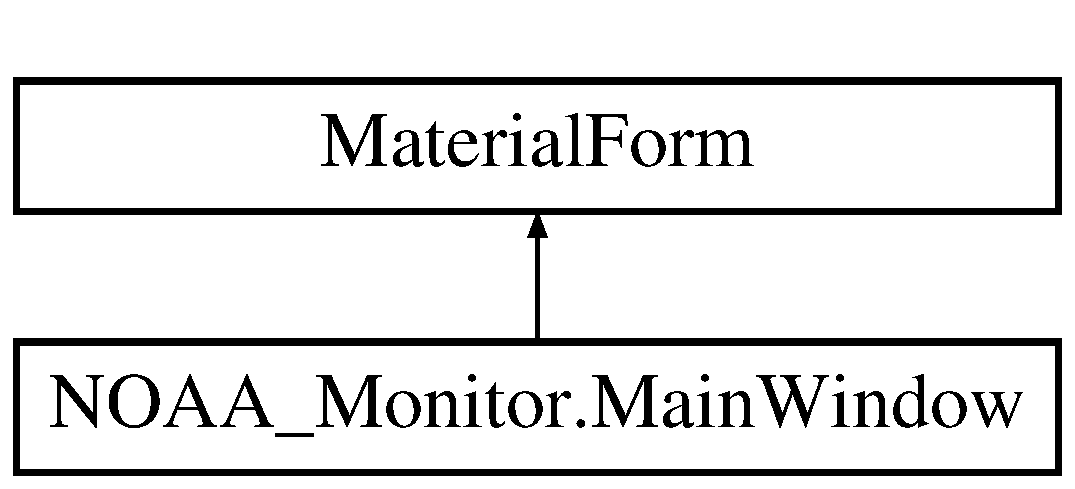
\includegraphics[height=2.000000cm]{class_n_o_a_a___monitor_1_1_main_window}
\end{center}
\end{figure}
\subsection*{Public Member Functions}
\begin{DoxyCompactItemize}
\item 
\mbox{\Hypertarget{class_n_o_a_a___monitor_1_1_main_window_a28afa0207b2f097c7cb2c7a897b0715e}\label{class_n_o_a_a___monitor_1_1_main_window_a28afa0207b2f097c7cb2c7a897b0715e}} 
string {\bfseries timestamp\+File} (string \+\_\+file\+Name)
\item 
\mbox{\Hypertarget{class_n_o_a_a___monitor_1_1_main_window_a482faa4bc10f2e2ec72efca039a404bc}\label{class_n_o_a_a___monitor_1_1_main_window_a482faa4bc10f2e2ec72efca039a404bc}} 
\mbox{\hyperlink{class_buoy_list}{Buoy\+List}} {\bfseries read\+Buoy\+Data} (string \+\_\+file\+Name)
\item 
\mbox{\Hypertarget{class_n_o_a_a___monitor_1_1_main_window_ab95ce7dd370e11ff7f4e4234bfd6f87b}\label{class_n_o_a_a___monitor_1_1_main_window_ab95ce7dd370e11ff7f4e4234bfd6f87b}} 
void {\bfseries change\+Station\+Picture} (string \+\_\+station\+Name)
\end{DoxyCompactItemize}
\subsection*{Public Attributes}
\begin{DoxyCompactItemize}
\item 
\mbox{\Hypertarget{class_n_o_a_a___monitor_1_1_main_window_abb42cf322b24155ae50b85f9132dbe26}\label{class_n_o_a_a___monitor_1_1_main_window_abb42cf322b24155ae50b85f9132dbe26}} 
Material\+Skin.\+Controls.\+Material\+Raised\+Button {\bfseries material\+Raised\+Button1}
\item 
\mbox{\Hypertarget{class_n_o_a_a___monitor_1_1_main_window_a5e7a69258252e7d3a865e6b2ecf7c61c}\label{class_n_o_a_a___monitor_1_1_main_window_a5e7a69258252e7d3a865e6b2ecf7c61c}} 
Material\+Skin.\+Controls.\+Material\+Raised\+Button {\bfseries material\+Raised\+Button2}
\end{DoxyCompactItemize}
\subsection*{Protected Member Functions}
\begin{DoxyCompactItemize}
\item 
override void \mbox{\hyperlink{class_n_o_a_a___monitor_1_1_main_window_ac64bbb0b9693f1395e5281805afe01b2}{Dispose}} (bool disposing)
\begin{DoxyCompactList}\small\item\em Clean up any resources being used. \end{DoxyCompactList}\end{DoxyCompactItemize}


\subsection{Member Function Documentation}
\mbox{\Hypertarget{class_n_o_a_a___monitor_1_1_main_window_ac64bbb0b9693f1395e5281805afe01b2}\label{class_n_o_a_a___monitor_1_1_main_window_ac64bbb0b9693f1395e5281805afe01b2}} 
\index{N\+O\+A\+A\+\_\+\+Monitor\+::\+Main\+Window@{N\+O\+A\+A\+\_\+\+Monitor\+::\+Main\+Window}!Dispose@{Dispose}}
\index{Dispose@{Dispose}!N\+O\+A\+A\+\_\+\+Monitor\+::\+Main\+Window@{N\+O\+A\+A\+\_\+\+Monitor\+::\+Main\+Window}}
\subsubsection{\texorpdfstring{Dispose()}{Dispose()}}
{\footnotesize\ttfamily override void N\+O\+A\+A\+\_\+\+Monitor.\+Main\+Window.\+Dispose (\begin{DoxyParamCaption}\item[{bool}]{disposing }\end{DoxyParamCaption})\hspace{0.3cm}{\ttfamily [inline]}, {\ttfamily [protected]}}



Clean up any resources being used. 


\begin{DoxyParams}{Parameters}
{\em disposing} & true if managed resources should be disposed; otherwise, false.\\
\hline
\end{DoxyParams}


The documentation for this class was generated from the following files\+:\begin{DoxyCompactItemize}
\item 
Form1.\+cs\item 
Form1.\+Designer.\+cs\end{DoxyCompactItemize}

\hypertarget{class_mapping}{}\section{Mapping Class Reference}
\label{class_mapping}\index{Mapping@{Mapping}}
\subsection*{Public Member Functions}
\begin{DoxyCompactItemize}
\item 
\mbox{\Hypertarget{class_mapping_a0b136ec61538a1e99eb9c267509207a4}\label{class_mapping_a0b136ec61538a1e99eb9c267509207a4}} 
{\bfseries Mapping} (string \+\_\+x\+Coordinate, string \+\_\+y\+Coordinate, string \+\_\+zoom\+Level=\char`\"{}0\char`\"{}, string \+\_\+map\+Mode=\char`\"{}T\+A2\char`\"{})
\item 
\mbox{\Hypertarget{class_mapping_a9112745f5e28c21780b47d4e74965c07}\label{class_mapping_a9112745f5e28c21780b47d4e74965c07}} 
void {\bfseries set\+New\+Map} (string \+\_\+map\+Mode)
\end{DoxyCompactItemize}
\subsection*{Properties}
\begin{DoxyCompactItemize}
\item 
\mbox{\Hypertarget{class_mapping_a51a982480ed02f06dfdf201227ebf012}\label{class_mapping_a51a982480ed02f06dfdf201227ebf012}} 
string {\bfseries map\+Mode}\hspace{0.3cm}{\ttfamily  \mbox{[}get, set\mbox{]}}
\item 
\mbox{\Hypertarget{class_mapping_a48aa705ccb646cc6bb3915ffd62fc8eb}\label{class_mapping_a48aa705ccb646cc6bb3915ffd62fc8eb}} 
string {\bfseries zoom\+Level}\hspace{0.3cm}{\ttfamily  \mbox{[}get, set\mbox{]}}
\item 
\mbox{\Hypertarget{class_mapping_afc902543b97a01af9bba71215ac36985}\label{class_mapping_afc902543b97a01af9bba71215ac36985}} 
string {\bfseries x\+Coordinate}\hspace{0.3cm}{\ttfamily  \mbox{[}get, set\mbox{]}}
\item 
\mbox{\Hypertarget{class_mapping_a4ea12d1c7dea2453d77a74811adcf8bc}\label{class_mapping_a4ea12d1c7dea2453d77a74811adcf8bc}} 
string {\bfseries y\+Coordinate}\hspace{0.3cm}{\ttfamily  \mbox{[}get, set\mbox{]}}
\item 
\mbox{\Hypertarget{class_mapping_ab5d51f857a9d569ffe7d9dea0830bbf6}\label{class_mapping_ab5d51f857a9d569ffe7d9dea0830bbf6}} 
string {\bfseries map\+U\+RL}\hspace{0.3cm}{\ttfamily  \mbox{[}get, set\mbox{]}}
\end{DoxyCompactItemize}


The documentation for this class was generated from the following file\+:\begin{DoxyCompactItemize}
\item 
Mapping.\+cs\end{DoxyCompactItemize}

%--- End generated contents ---

% Index
\backmatter
\newpage
\phantomsection
\clearemptydoublepage
\addcontentsline{toc}{chapter}{Index}
\printindex

\end{document}
